\documentclass[paper=a4,fontsize=11pt]{article}

%%%%%% Import Package %%%%%%
\usepackage{graphicx}
\usepackage[unicode]{hyperref}
\usepackage{cite}
\usepackage{indentfirst}
\usepackage{multirow}
\usepackage{indentfirst}
\usepackage{titlesec}
\usepackage{color}
\usepackage{listings}
\usepackage{fontspec,xunicode,xltxtra}
\usepackage{xeCJK}
\usepackage{hyperref}
\usepackage{enumerate}

%When compile under liunx% 
%\setmainfont{WenQuanYi Micro Hei}  
 
\definecolor{orange}{RGB}{255,127,0} 
\definecolor{SpringGreen4}{RGB}{0,139,69}

\renewcommand{\figurename}{图}
\renewcommand{\tablename}{表}

%%%% Set section Attribute %%%%
\makeatletter
\makeatother

%%%% 设置 subsection 属性 %%%%
\makeatletter
\makeatother

%%%% 设置 subsubsection 属性 %%%%
\makeatletter
\makeatother

%Set Hyperref Format
\hypersetup{pdfborder={0 0 0}, colorlinks=true,linkcolor=blue}

% 段落首行缩进两个字 %
\makeatletter
\let\@afterindentfalse\@afterindenttrue
\@afterindenttrue
\makeatother

\setlength{\parindent}{2em}  %中文缩进两个汉字位

%%%% 下面的命令重定义页面边距,使其符合中文刊物习惯 %%%%
\addtolength{\topmargin}{-54pt}
\setlength{\oddsidemargin}{0.63cm}  % 3.17cm - 1 inch
\setlength{\evensidemargin}{\oddsidemargin}
\setlength{\textwidth}{14.66cm}
\setlength{\textheight}{24.00cm}    % 24.62

%%%% 下面的命令设置行间距与段落间距 %%%%
\linespread{1.4}
% \setlength{\parskip}{1ex}
\setlength{\parskip}{0.5\baselineskip}

%Set where to find the graphics%
\graphicspath{{./Image/}{./Image/FormDesign/}{./Image/InterfaceDesign/}}
%\graphicspath{{I:\Nutstore\Document\Tex\JsptpdCSSDS\Image\Interface\_Design}}%

%Set Code Format%
\lstloadlanguages{C, csh, make}
\lstset{	
	language=C
	,tabsize=4
	,keepspaces=true
	,breakindent=22pt
	,numbers=left
	,stepnumber=1
	,numberstyle=\tiny
	,basicstyle=\footnotesize
	,showspaces=false
	,flexiblecolumns=true
	,breaklines=true
	,breakautoindent=true
	,breakindent=4em
	,escapeinside={/*@}{@*/}
}

%%%% 正文开始 %%%%
\begin{document}
	%%%% 定义标题格式,包括title,author,affiliation,email等 %%%%
	\title{开源软件介绍}		
	\author{蒋小强\footnote{mail:jiangtingqiang@gmail.com}}
	\date{2015.03}	
	
	%%%% Generate Title %%%%  
	\maketitle %
	\clearpage
	
	\begin{table}\caption{修改记录}					
		\medskip
		\centering		
		\begin{tabular}{|c|c|c|c|c|}
			\hline
			\multirow{1}{*}{序号}
			& \multicolumn{1}{|c|}{修改人}  
			& \multicolumn{1}{|c|}{修改日期} 
			& \multicolumn{1}{|c|}{备注}\\			
			\cline{1-4}
			1 & 蒋小强 & 2014-10-22 & 创建基础版本\\
			\hline
			2 & & &\\
			\hline
			3 & & &\\
			\hline
			4 & & &\\
			\hline
		\end{tabular}
	\end{table}
	\clearpage
	\section{前言}
	%Preamble
	
	记得小时候小伙伴有小吃,也会分给我一颗。潜移默化的在将来生活中也会考虑到一起生活的朋友。分享是妙不可言的,特别是有同样认知的朋友,咦,你也喜欢听这首音乐!但是对于使用的软件,或许大家并不是太留意。大家的电脑都装着360,装着QQ。我想软件也是需要分享的,一款优秀的软件让人爱不释手,臭虫不断的软件真是噩梦。在商业化时代的今天,我相信开源软件有它的价值,其实开源软件一直伴随着我们,只是我们没有意识到而已。腾讯的QQ、多数播放器(QQ影音、暴风影音....)、迅雷、大部分的浏览器、网站及数据库等。如果现在需要开发一款产品,首先想到的是找一块类似的开源实现版本,然后在原有的基础上修改,即可推向商业市场,极少有例外。热爱分享,热爱开源,同时也意识到一款优秀的软件倾注了太多的普通人甚至是业人士无法想象的时间和精力。开源没有想象中的美好,有利有弊,但是如果没有开源的贡献,现在的软件行业或许是另一番景象。	
	
	如今的软件都变得相当臃肿,我们真的需要那么多的功能吗?我们能够选择使用哪些功能吗?目前的软件使用到全部功能的10\%就已经非常可观了。在我的心目中,软件应该是简单、专注、小巧、干净,而不是复杂臃肿、各种功能、庞大、各种不知名的弹窗,不明所以的文件。而目前的绝大部分商业软件都是夹带商业目的,与软件需要完成的功能背道而驰。为了商业目的而舍弃原则,采用所谓的“下三滥\footnote{包括后台静默安装、强制安装,利用隐蔽的选项诱导安装,扎人眼球的广告推广,后台监听进程或者服务且服务无法删除或者卸载}”的手段进行推广。并非反对利用软件赚钱,一款优秀的软件所投入的资金和时间是无法想象的,甚至是不能简单用金钱可以衡量。但是绝大多数软件却是“强迫性”的,只有选项“是”,没有“否”的选项,内行人一看就明白,这是一个不好的现象。
	
	
	
	\newpage
	\section{总览}
	
	\subsection{开源协议}
	
	\subsubsection{GNU}
	
	
	
	\clearpage
	
	\part{基础软件}
	
	基础软件包括操作系统、数据库系统、中间件、语言处理系统(包括编译程序、解释程序和汇编程序)和办公软件(包括文字处理、电子表格、幻灯片以及一些初级图片处理程序)。
		
	\clearpage
	
	当购买电脑时,最重要的就是为新买的爱机安装操作系统了,最熟悉的当属微软的Windows视窗操作系统,但这里不准备花费太多笔墨来推荐它,事实上我不推荐安装Windows操作系统,但是仅仅只有极少数人真正把忽视Windows放在心里,因为现在Windows在大众中应用太普遍了,忽视它已然无法做到。事实上Windows操作系统可以称的上是软件工程里的一个典范,到目前为止我想它真正的无法衡量它的价值了,如果再从头开发Windows操作系统,无法想象。笔者真正感兴趣的是由Linus Benedict Torvalds组织开发的基于Linux内核的各种发行版本。
	
	\newpage
	
	\section{Slackware}
	
	\subsection{USB}
	
	安装完毕Slackware后,读取U盘时可能会遇到如下错误:A security policy in place prevents this sender from sending this message to this recipient, see message bus configuration file (rejected message had interface “org.freedesktop.Hal.Device.Volume” member “Mount” error name “(unset)” destination “org.freedesktop.Hal”),如图\ref*{USBSecurityError}所示。
	\begin{figure}[htbp]
		\centering
		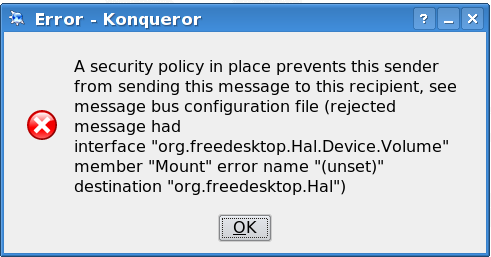
\includegraphics[scale=0.7]{USBSecurityError.png}
		\caption{打开USB设备错误}
		\label{USBSecurityError}
	\end{figure}
	导致此问题的原因是:This is caused by the hal daemon not allowing you to access the device because of a security policy. The hal daemons security policy resides in a file at “/etc/dbus-1/system.d/hal.conf”\footnote{http://www.jefferyfernandez.id.au/2007/07/26/a-security-policy-in-place-prevents-mounting-of-volumes/}. 解决的办法是将root添加到plugdev用户组中。
	\begin{enumerate}
		\setcounter{enumi}{0}
		\item{\textbf{查看所有的用户和用户组}}
		
		groups
		
		\item{\textbf{将用户添加到组}}
		
		此处需要将root用户添加到组plugdev中。键入命令:
		\begin{lstlisting}
		usermod -G plugdev root
		gpasswd -a root plugdev
		\end{lstlisting}
		或者将用户从组中删除:
		\begin{lstlisting}
		gpasswd -d root plugdev
		\end{lstlisting}
		
		\item{\textbf{重启计算机}}
		
		reboot
		
		hal daemon的路径为:/usr/sbin/hald。
		
	\end{enumerate}
	
	\subsection{修改引导等待时间}
	
	slackware用的bootloader是lilo,等待时间长达2分钟,需要回车才能继续起动,不是很方便,更改启动等待时间如下。
	
	1.将prompt注释掉,加入compact
	
	2.将timeout = 1200 改为timeout = 3
	
	3.退出后在命令行输入: lilo -v,这样下次就直接启动了.
	
	\subsection{修改CMD界面屏幕分辨率}
	
	由于slackware使用的是LILO进行引导系统的启动,因此配置分辨率的文件为/ect/lilo.conf。通过修改lilo.conf文件中的vga的参数即可。例如:
	
	\# 1028*768*256 
	vga=790 
	
	\# 800*600*256
	vga=787
	
	\# 640*480*256
	vga=784
	
	配置完成后,运行lilo -v命令后重启计算机即可。
	
	说明:配置适合的分辨率才能正常显示,否则系统会使用默认的分辨率,不合适的分辨率会导致屏幕变花,此时只要进入命令行界面修改为合适分辨率之后屏幕即可正常显示。
	
	\subsection{挂载U盘}
	
	列出当前磁盘分区,如图\ref{fdisklist}所示。
	
	fdisk -l
	
	\begin{figure}[htbp]
		\centering
		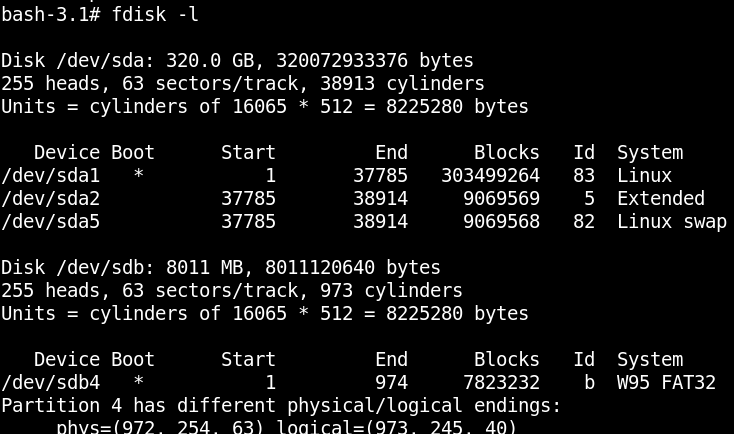
\includegraphics[scale=0.5]{fdisklist.png}
		\caption{列出当前磁盘分区}
		\label{fdisklist}
	\end{figure}
	
	在mnt目录下新建文件夹,用于挂载的目的文件夹。键入挂载命令,如图\ref{mountusbdisk}所示。
	
	mount /dev/sdb4 /mnt/usb
	
	\begin{figure}[htbp]
		\centering
		
\includegraphics[scale=0.7]{mountusbdisk.png}
		\caption{挂载USB}
		\label{mountusbdisk}
	\end{figure}
	
	
	
	
	
	
	\subsection{网络配置}
	
	\subsubsection{基础命令}
	
	\noindent ifconfig -a查看当前可用的所有的网卡\newline
	ifconfig查看当前能用的网卡
	
	
	
	
	\subsubsection{配置步骤}
	
	\paragraph{查看网卡名称}
	在命令行模式下键入lspci|grep -i eth命令,列出的网卡名称为:Silicon Integrated Systems SiS 191 Gigabit Ethernet Adapter。
	
	\paragraph{下载网卡驱动}
	到http://w3.sis.com/download/下载Linux下的网卡驱动,如图\ref{DownloadSisDriver}所示。
	\begin{figure}[htbp]
		\centering
		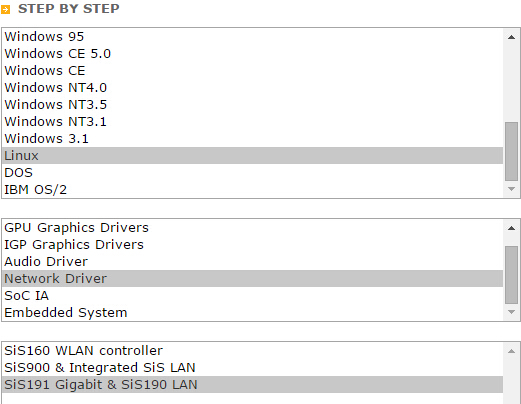
\includegraphics[scale=0.7]{DownloadSisDriver.jpg}
		\caption{驱动选择}
		\label{DownloadSisDriver}
	\end{figure}
	
	
	\paragraph{编译网卡驱动}
	编译网卡驱动参照下载的源码包里面的readme.txt文件操作。
	\begin{enumerate}
		\setcounter{enumi}{0}
		\item{\textbf{将源文件拷贝到指定目录下~~}}
		
		cp sis190.c /usr/src/linux-2.6.9/drivers/net
		
		\item{\textbf{编辑配置文件~~}}
		
		Edit the file "/usr/src/linux-2.6.9/drivers/net/Kconfig".
		a. Serach for the string "config SIS900"
		b. Add the following item below the item of SIS190.
		
		config SIS190\newline
		tristate "SiS 191/190 PCI Gigabit/Fast Ethernet Adapter support"\newline
		depends on NET\_PCI \&\& PCI\newline
		select CRC32\newline
		---help---\newline
		Say Y here if you have a SiS 191/190 PCI Gigabit/Fast Ethernet adapter.
		
		To compile this driver as a module, choose M here: the module
		will be called sis190.  This is recommended.
		
	\end{enumerate}
	
	\subsubsection{rc.inet1}
	/etc/rc.d/rc.inet1
	\subsubsection{ifconfig}
	
	\section{Ubuntu}
	
	\subsection{ASUS F81se安装Ubuntu 12.04 LTS}
	
	\subsection{设置Ubuntu待机时机}
	
	\subsection{安装中文输入法}
	
	\begin{enumerate}
		\setcounter{enumi}{0}
		\item{\textbf{查看所有的用户和用户组}}
		\item{\textbf{安装Ibus框架}}~~调出terminal终端,输入:sudo apt-get install ibus ibus-clutter ibus-gtk ibus-gtk3 ibus-qt4
		
		启动Ibus框架:im-switch -s ibus
		
		安装Ibus框架完成之后,需要注销或者重启系统使Ibus生效。
		\item{\textbf{安装拼音引擎}}~~有很多拼音引擎可供选择,一般安装一种就够了,比如我就直接安装的第一种\newline
		
		Ibus 拼音:sudo apt-get install ibus-pinyin\newline
		
		Ibus 五笔:sudo apt-get install ibus-table-wubi\newline
		
		Google 拼音:sudo apt-get install ibus-googlepinyin\newline
				
		Sun 拼音:sudo apt-get install ibus-sunpinyin
				
		\item{\textbf{设置Ibus框架}}~~在 terminal 中输入命令:ibus-setup,系统调出Ibus设置界面,如图\ref{IbusSetup}所示。选择Tab页中的Input Method,设置Google Pinyin,如图\ref{IbusSetupGooglePinyin}所示。
		
		\begin{figure}[htbp]
			\centering
			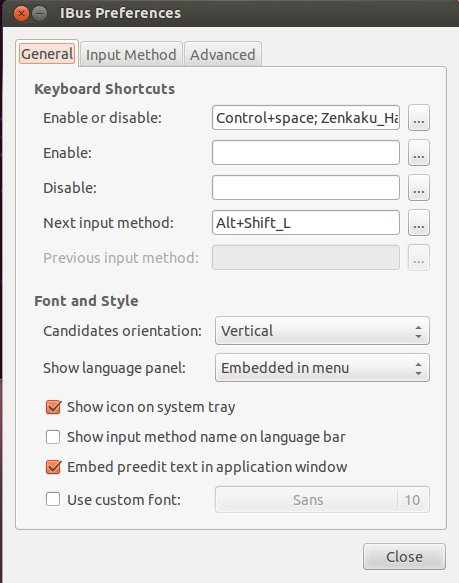
\includegraphics[scale=0.7]{IbusSetup.jpeg}
			\caption{Ibus设置界面}
			\label{IbusSetup}
		\end{figure}
		
		\begin{figure}[htbp]
			\centering
			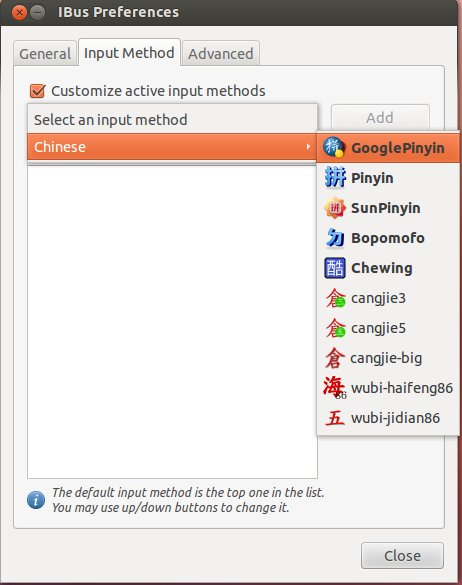
\includegraphics[scale=0.7]{IbusSetupGooglePinyin.jpeg}
			\caption{Ibus input method设置}
			\label{IbusSetupGooglePinyin}
		\end{figure}
		
		
	\end{enumerate}
	
	\subsection{Git}
	
	查看是否已经安装Git:git --version.
	如果没有安装git,键入命令:sudo apt-get install git git-core 安装git
	
	
	\section{LaTex}
	
	\subsection{安装xeCJK}
	
	sudo apt-get install latex-cjk-xcjk cjk-latex latex-cjk-chinese
	
	\clearpage
		
	\part{工具}
	
	\clearpage
	
	\section{下载工具}	
	\subsection{aMule}
	aMule stands for all-platform Mule.aMule is an eMule-like client for the eD2k and Kademlia networks, supporting multiple platforms.Currently aMule (officially) supports a wide variety of platforms and operating systems, being compatible with more than 60 different hardware+OS configurations.aMule is entirely free, its sourcecode released under the GPL just like eMule, and includes no adware or spyware as is often found in proprietary P2P applications.aMule is built upon the wxWidgets (formerly wxWindows) toolkit, which enables it to support multiple platforms.
	\subsubsection{为什么使用aMule}
	使用aMule主要基于以下原因:
	\begin{itemize}
		\item{它是开源软件}
		\item{它很简单}
		\item{它很小巧}
	\end{itemize}
	
	\subsubsection{eD2k链接}

	\paragraph{基本的 eD2k 链接}
	ed2k://|file|<文件名称>|<文件大小>|<文件哈希值>|/一个 eD2k链接包含必要的文件描述像是名称, 大小及哈希值形成基本的格式
	
	\subsubsection{为何aMule会有HighID、LowID之分}
	
	无论什么类型的P2P软件,MSN、QQ、BT……都无法实现两个内网用户——LowID用户之间的直接通讯。MSN、QQ等即时聊天工具都是通过服务器转发数据实现的,像MSN,所有的数据都是通过服务器转发,因此MSN上是看不到好友的IP地址的。而如果你用过早期QQ版本的话,应该知道有一种情况经常会发生,就是即使聊天的2个人都在线,所有的聊天内容后面都会跟上“(通过服务器转发)”,现在的版本只是已经去掉了这句话。然而,为传输大量数据而设计的eMule、BT等P2P软件显然无法使用“服务器转发”来实现LowID用户之间的通信——因为大量的数据转发会无端浪费极大的网络带宽,并且eMule、BT之类免费软件也无法提供要求如此之高的服务器来完成这项任务。BT之中没有LowID的说法只是因为它不提,而不是它能够解决这个问题。所以不要说因为LowID的关系而放弃eMule转用BT,那是荒诞无稽的笑话:-)
		
	\subsubsection{aMule的配置}
	在下载好aMule之后,启动后会提示获取了Low ID\footnote{Low ID一般都是没有公网IP的内网用户,两个Low ID用户之间是无法直接连接的,所以Low ID的用户下载源会相对少一点(无法从其它Low ID用户那里下载)。}。如何获取High ID\footnote{High ID就是拥有独立公网IP并且能提供端口(默认4662)给eMule工作的用户;此类用户可以和任何eMule兼容客户端连接与下载。}呢?只需要设置路由的转发规则和将本机设置为DMZ主机2个步骤即可\footnote{http://www.emule.org.cn/topic/lowid/}。获取HignID之后界面显示如图\ref{GetHighID}所示。
	
	\begin{figure}[htbp]
		\centering
		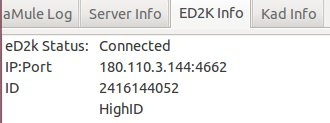
\includegraphics[scale=0.8]{GetHighID.jpeg}
		\caption{HighID显示}
		\label{GetHighID}
	\end{figure}
	
	\begin{enumerate}
		\setcounter{enumi}{0}
		\item\textbf{{设置路由的转发规则~~}}
		如果您的机器在局域网内,那么需要添加数据包转发规则以及将本机设置为DMZ主机,转发规则的设置如图\ref{RouterTransportRule}所示。填写的参考如图\ref{aMulePortParameter}所示。	
		\begin{figure}[htbp]
			\centering
			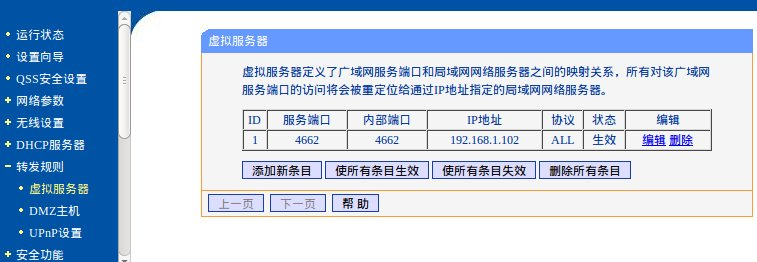
\includegraphics[scale=0.5]{RouterTransportRule.jpeg}
			\caption{设置路由转发规则}
			\label{RouterTransportRule}
		\end{figure}
		
		\begin{figure}[htbp]
			\centering
			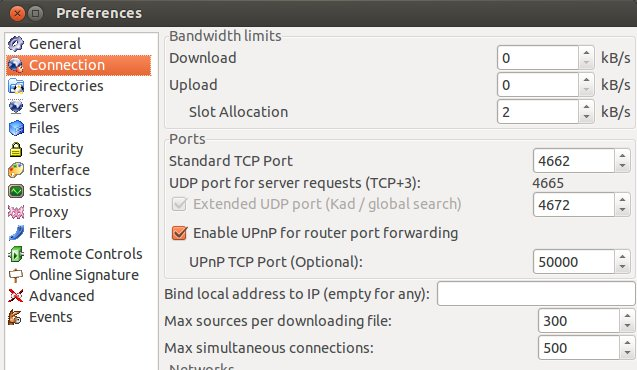
\includegraphics[scale=0.5]{aMulePortParameter.jpeg}
			\caption{aMule端口}
			\label{aMulePortParameter}
		\end{figure}
		
		\item{\textbf{设置DMZ主机~~}}
		设置DMZ主机如图\ref{SetDMZServer}所示。
		\begin{figure}[htbp]
			\centering
			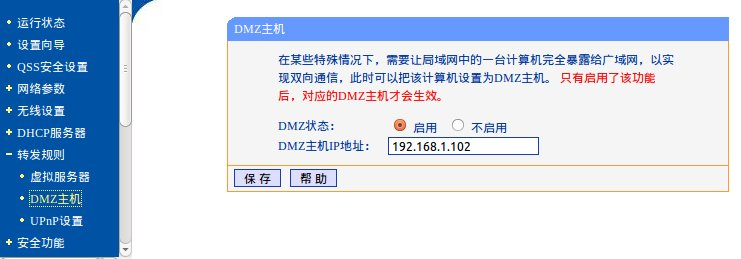
\includegraphics[scale=0.5]{SetDMZServer.jpeg}
			\caption{设置DMZ主机}
			\label{SetDMZServer}
		\end{figure}
		
	\end{enumerate}
	
	\subsection{Deluge}
	\subsubsection{简介}
	Deluge is a full-featured ​BitTorrent client for Linux, OS X, Unix and Windows. It uses ​libtorrent in its backend and features multiple user-interfaces including: GTK+, web and console. It has been designed using the client server model with a daemon process that handles all the bittorrent activity. The Deluge daemon is able to run on headless machines with the user-interfaces being able to connect remotely from any platform.
	
	Deluge features a rich plugin collection; in fact, most of Deluge's functionality is available in the form of plugins.
	
	Deluge was created with the intention of being lightweight and unobtrusive. It is our belief that downloading shouldn't be the primary task on your computer and therefore shouldn't monopolize system resources.
	
	Deluge is not designed for any one desktop environment and will work just fine in GNOME, KDE, XFCE and others. We do our best to adhere to the ​freedesktop standards.
	
	Deluge is ​Free Software and is licensed under the ​GNU General Public License.
	
	
	\begin{figure}[htbp]
		\centering
		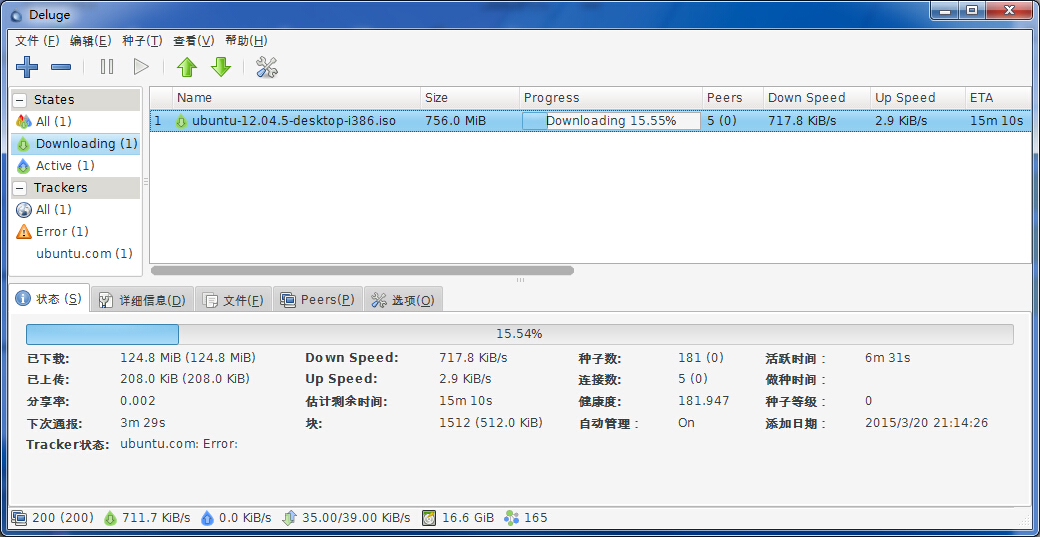
\includegraphics[scale=0.35]{DelugeWindowsUI.jpg}
		\caption{Deluge主界面}
		\label{DelugeWindowsUI}
	\end{figure}
	
	\subsection{Open Download Manager}
	
			
	
	\section{KSnapshot}
	
	\subsection{简介}
	
	KSnapshot is a simple application for taking screenshots. It is capable of capturing images of the whole desktop, a single window, a section of a window, a selected rectangular region or a freehand region. The images can then be saved in a variety of formats.
	
	\subsection{使用}	
	
	在Ubuntu下使用快捷键Ctrl+Alt+T打开终端,输入命令ksnapshot\footnote{事实上可以切换到/usr/bin目录下,此目录已经在环境变量中,此目录下的可运行程序皆可以通过命令的方式打开。}即可打开。
	

	
	\section{Mozilla Thunderbird}
	
	\subsection{简介}
	
	Mozilla Thunderbird是由Mozilla浏览器的邮件功能部件所改造的邮件工具,使用 XUL 程序界面语言所设计,是专门为搭配 Mozilla Firefox 浏览器使用者所设计的邮件客户端软件,介面设计更简洁、而且免安装。 这款软件非常优秀,目前官方最新版本为 24.5.0,早期版本有 2.0.0.24 和 3.1.17。2.x 和 3.1.x 系列的后台资源占用很低,适合配置不高的用户;9.0.x 系列资源占用较高但数据安全性有了很大提高,功能也更加丰富。
	
	Thunderbird is a free email application that's easy to set up and customize - and it's loaded with great features!
	
	\section{即时同讯}	
	
	\subsection{Pidgin}	
	
	\subsubsection{简介}
	
	Pidgin (formerly named Gaim) is an open-source multi-platform instant messaging client, based on a library named libpurple. Libpurple has support for many commonly used instant messaging protocols, allowing the user to log into various services from one application.
	The number of Pidgin users was estimated to be over 3 million in 2007.\footnote{http://en.wikipedia.org/wiki/Pidgin\_(software)}
	
	Pidgin的主界面如图\ref{PidginWebQQMainUI}所示。聊天界面如图\ref{PidginWebQQTalking}所示。
	\begin{figure}[htbp]
		\centering
		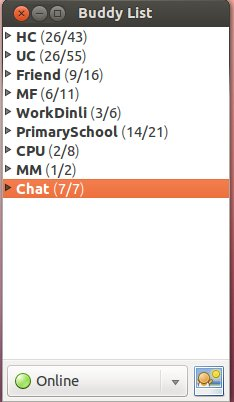
\includegraphics[scale=0.8]{PidginWebQQMainUI.jpeg}
		\caption{Pidgin主界面}
		\label{PidginWebQQMainUI}
	\end{figure}
	
	\begin{figure}[htbp]
		\centering
		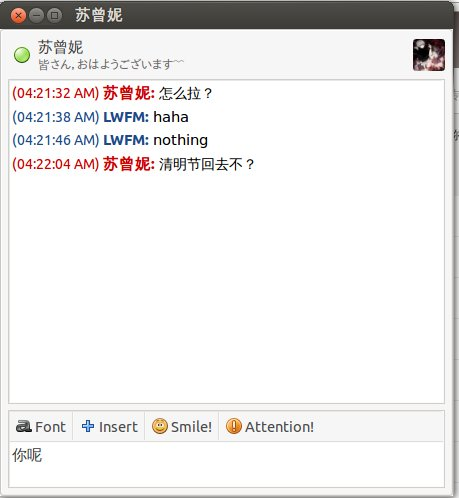
\includegraphics[scale=0.8]{PidginWebQQTalking.jpeg}
		\caption{Pidgin聊天界面}
		\label{PidginWebQQTalking}
	\end{figure}	
	
	\section{其他工具}
	
	\subsection{LICEcap}
	
	\subsubsection{简介}
	
	LICEcap can capture an area of your desktop and save it directly to .GIF (for viewing in web browsers, etc) or .LCF (see below). 
	
	LICEcap is an intuitive but flexible application (for Windows and now OSX), that is designed to be lightweight and function with high performance. 
	
	LICEcap is easy to use: view a demo (output is here). 
	
	In addition to .GIF, LICEcap supports its own native lossless .LCF file format, which allows for higher compression ratios than .GIF, higher quality (more than 256 colors per frame), and more accurate timestamping. If you record to .LCF, you can play back the .LCF files within REAPER (and/or use it to convert to .gif or another video format). 
	
	LICEcap is GPL free software, each download package includes the source. 
	
	Features and options:
	Record directly to .GIF or .LCF.
	Move the screen capture frame while recording.
	Pause and restart recording, with optional inserted text messages.
	Global hotkey (shift+space) to toggle pausing while recording
	Adjustable maximum recording framerate, to allow throttling CPU usage.
	Basic title frame, with or without text.
	Record mouse button presses.
	Display elapsed time in the recording.
	Requirements:
	For Windows: Windows XP/Vista/7/8/8.1 (might work with reduced functionality on other versions)
	For OSX: OS 10.4+ (10.6+ for full feature support), PPC or Intel (note: OS X support is still preliminary, some features are not supported)
	A reasonably fast CPU
	A healthy amount of RAM (1GB+, especially when encoding to LCF)
	
	\subsection{Adblock Plus}
	
	\subsubsection{简介}
	
	Adblock Plus lets you block annoying ads, tracking, malware and other things you may not want in your browser. Adblock Plus is an open source project created by Wladimir Palant in 2006. Eyeo was founded in 2011 by Wladimir Palant and Till Faida to make its development sustainable.
	
	
	\subsection{优点}
	
	有的时候浏览网页时,时不时会弹出美女的照片,然后就不假思索的点击了,但是点出来却是“延时广告”(你懂的),屡次如此觉得自己受到欺骗了。不反对弹出美女图片,甚至我非常喜欢性感美女照片(谁不喜欢呢),但是利用美女来诱惑我点击是我不能容忍的,我么有得到任何对我有用的内容,如果您也有同样的问题,那么Adblock Plus是一个非常好的选择。	
	
	
	\subsection{Shutter}
	
	\subsubsection{简介}
	
	Shutter is a feature-rich screenshot program for Linux based operating systems such as Ubuntu. You can take a screenshot of a specific area, window, your whole screen, or even of a website – apply different effects to it, draw on it to highlight points, and then upload to an image hosting site, all within one window. Shutter is free, open-source, and licensed under GPL v3.	
	
	\subsection{WinDirStat}
	
	\subsubsection{简介}
	WinDirStat is a disk usage statistics viewer and cleanup tool for various versions of Microsoft Windows.
	
	在用Windows操作系统时C盘经常是越用越少,有时我们需要查看磁盘到底哪些文件最占用空间,占用空间的比重,以便于有针对性的清理。记得有一次我的磁盘莫名其妙的空间慢慢变少,几十个GB就慢慢的被占满,到最后才发现是Windows服务不停的向磁盘里写入日志,如果有这个工具的话,发现它就易如反掌了。
		
	\subsection{KDirStat}
	KDirStat is a graphical disk usage utility, very much like the Unix "du" command. In addition to that, it comes with some cleanup facilities to reclaim disk space.
	
	While KDirStat is a KDE program, it runs fine on every X11 desktop, i.e., it runs on Linux, BSD, and lots of other Unix-type systems (Solaris, HP-UX, AIX, ...).
	
	MS Windows Users please note that there are operating systems and window systems beyond those from Redmond, WA. This may come as a surprise to some people. ;-) There is a MS Windows clone called WinDirStat. Yes, that one is the clone. KDirStat is the original.
		
	\subsection{i2p}
	
	I2P是洋文 Invisible Internet Project 的缩写。官方网站是 http://www.i2p2.de/。I2P 在很多方面跟 TOR 相似——也是开源软件、也采用分布式、也强调隐匿性。I2P 项目成立于2003 年,是一个在匿名网络环境下进行安全数据传输的框架,数据在传输的过程中经过了多层次的加密。和tor不同的是它没有中央服务器,而是通过用户组成分布式 网路,实现匿名加密访问的网络。
	
	\subsection{Tor}
	
	Tor is free software and an open network that helps you defend against traffic analysis, a form of network surveillance that threatens personal freedom and privacy, confidential business activities and relationships, and state security.
	
	
	\subsection{audacity}
	
	A fast, cross-platform audio editor
	
	\clearpage
	
	\part{娱乐}
	
	\clearpage
	
	\section{VLC Media Player}	
	
	\subsection{简介}
	VLC is a renowned media player that works with most multimedia files and DVDs, audio CDs, VCDs, and various streaming protocols. VLC is so well respected that it’s the go to media player for downloads that won’t play in its commercial counterparts. It is also a compelling server that streams live and on-demand video, through both IPv4 and IPv6 protocols, on a high-bandwidth network. VLC’s versatility, advanced controls, and broad support for numerous file types make it a popular choice for media playback and conversion worldwide. 
	
	VLC多媒体播放器具有跨平台的特性,它有Linux、Microsoft Windows、Mac OS X、BeOS、BSD、Pocket PC及Solaris的版本。
	
	与另一个著名播放器Mplayer(使用Gtk+库)不同的是,VLC使用了Qt库来编写Linux的用户操作界面。
	
	在Windows,Linux以及某些平台,VLC提供了一个Mozilla扩充包,使得某些网站上附带的QuickTime及Windows Media多媒体文件,可以在非微软或苹果计算机的操作系统中,正常显示于Mozilla的浏览器下。
	
	从版本0.8.2开始,VLC亦提供了一个ActiveX的扩充包,使用户可以在Internet Explorer下,正常显示某些网站上附带的QuickTime及Windows Media多媒体文件。
	从1.0.5版本开始VLC的ActiveX的扩充包已经放弃js接口的调用。
	VLC还有一个非常好的功能——支持播放某些没有下载完成的视频文件部份内容。
	
	\section{Qmmp}
	
	\subsection{简介}
	qmmp is a free and open-source audio player written in C++ with the help of the Qt library. It officially supports the operating systems Linux, FreeBSD and Microsoft Windows. It is the only audio player not featuring a database that uses the Qt library.
	
	\section{射手影音}
	
	\subsection{简介}
	射手影音播放器是由射手网创建与维护的开源播放器项目。内核基于MPC、MPC-HC和ffmpeg。同时加入更多真正符合中国用户习惯的功能,旨在改进华人的数字影视观赏体验,建立和维护一个真正属于中文用户的开源播放器。
	
	信奉信息自由,交流创造价值。作者很长一段时间以来,对手头的播放器颇为不满意:领先的播放器技术都是国外的,而国内的所谓播放器,不仅被插件插的一塌糊涂,还将海外的开源播放器拿回来打个包,就挂上自己的名字开始糟蹋别人的GPL。
	
	所以在2008年末,这个华人播放器开源项目在沈晟的带领下启动了,旨在为华人的使用习惯,来尽量做得最好,而且尊重和遵守开源协议。
			
	\section{SuperTuxKart}
	
	\subsection{简介}
	
	SuperTuxKart, also known as STK, is a free and open-source kart racing video game featuring the Linux mascot Tux. SuperTuxKart is cross-platform, running on Windows, Mac OS, Linux, AmigaOS 4, AROS, MorphOS and other Unix systems. The latest stable version of the game is version 0.8.1 and was released on November 26, 2013. On December 17, 2014, the development team released a beta version of SuperTuxKart 0.8.2, which featured an all new graphics engine.
	
	\subsection{道具说明}
	
	\noindent 泡泡糖:产生大泡泡来保护你,或者向后看时使用,你身后留下泡泡糖,经过泡泡糖的车辆速度会迅速降低\newline
	蛋糕:自动瞄准离你最近的敌人,并扔出可以爆炸的蛋糕,适合于短距离或正前方的对手\newline
	马桶揣子:向前看时射出马桶揣子,如果成功吸住墙壁或其他车辆可使自己加速,若吸住其他车辆还可使被吸住车辆减速;向后看时射出马桶揣子,被射中者视线将会受到影响\newline
	保龄球:扔出保龄球以攻击其他车辆,向后看时使用则向后扔\newline
	降落伞:可减缓所有在你前面的车的速度\newline
	锚:可使位于第一名的车辆速度瞬间变为0\newline
	魔法箱子:使得箱子和香蕉皮,氮气和泡泡糖在短时间内暂时颠倒\newline
	烂篮球:会自动跳到第一名那里并炸飞第一名,同时压扁被它弹到的车,使他们减速。注:它碰到墙就会爆炸,或用蛋糕也可以把它炸掉。\newline
	苍蝇拍:会拍扁附近的赛车,使他们减速。如自己车上有定时炸弹的话,它可以拍飞定时炸弹。\newline
	加速器:可在短时间内使你的赛车加速\newline
	氮气:收集氮气作为燃料,当你按键使用它时可以获得很大的加速度\newline
	以上道具,除了氮气,都可以通过收集蓝色宝箱来获得。\newline
	在常规比赛和竞速模式中路上会出现香蕉皮和泡泡糖,要尽量避开,碰到香蕉皮会被惩罚,而碰到泡泡糖则会减速。\newline
	香蕉的惩罚:\newline
	减速伞:减你自己的速度\newline
	定时炸弹:指针归零时炸弹爆炸。若在炸弹爆炸前再次撞上香蕉皮或撞上同样携带定时炸弹的车辆时,则炸弹立即爆炸。如自己车上有定时炸弹的话,撞别的车辆可以把定时炸弹撞到别的车身上。\newline
	锚:可使你的车辆速度瞬间变为0
	
	\clearpage
		
	\part{办公}
	
	\clearpage
	
	\section{GoldenDict}
	
	\subsection{简介}
	
	GoldenDict 是一款不错的、与StarDict(星际译王)类似的词典软件。它使用 WebKit作为渲染核心,格式化、颜色、图像、链接等支持一应俱全;支持多种词典文件格式,包括Babylon 的 .BGL 文件、StarDict 的 .ifo/.dict/.idx/.syn 文件、Dictd 的·index/.dict(.dz) 文件、ABBYY Lingvo 的 .dsl/.lsa/.dat 文件;
	
	GoldenDict可查询Wikipedia、Wiktionary 等基于 MediaWiki 的 Wiki 网站,且能够通过模板 Url模式来使用其他的在线词典网站;具有基于 Hunspell 的 morphology 系统;包含完整的 Unicode支持、scan 弹窗及全局热键等功能。
	
	GoldenDict 发布于 GNU GPLv3+ 许可之下,可运行于 Linux 和 Windows平台,其安装文件在这里能够找到。
	
	\subsection{词典列表}
	
	Oxford Advanced Learner's Dictionary 8th edition(En-En)-牛津高阶词典(英英)第8版
	
	Merriam-Webster's Collegiate 11th edition(En-En)-韦氏大学词典(英英)第11版,含图片及发音,如图\ref{GoldenDictWebster}所示。    
	
	\begin{figure}[htbp]
		\centering
		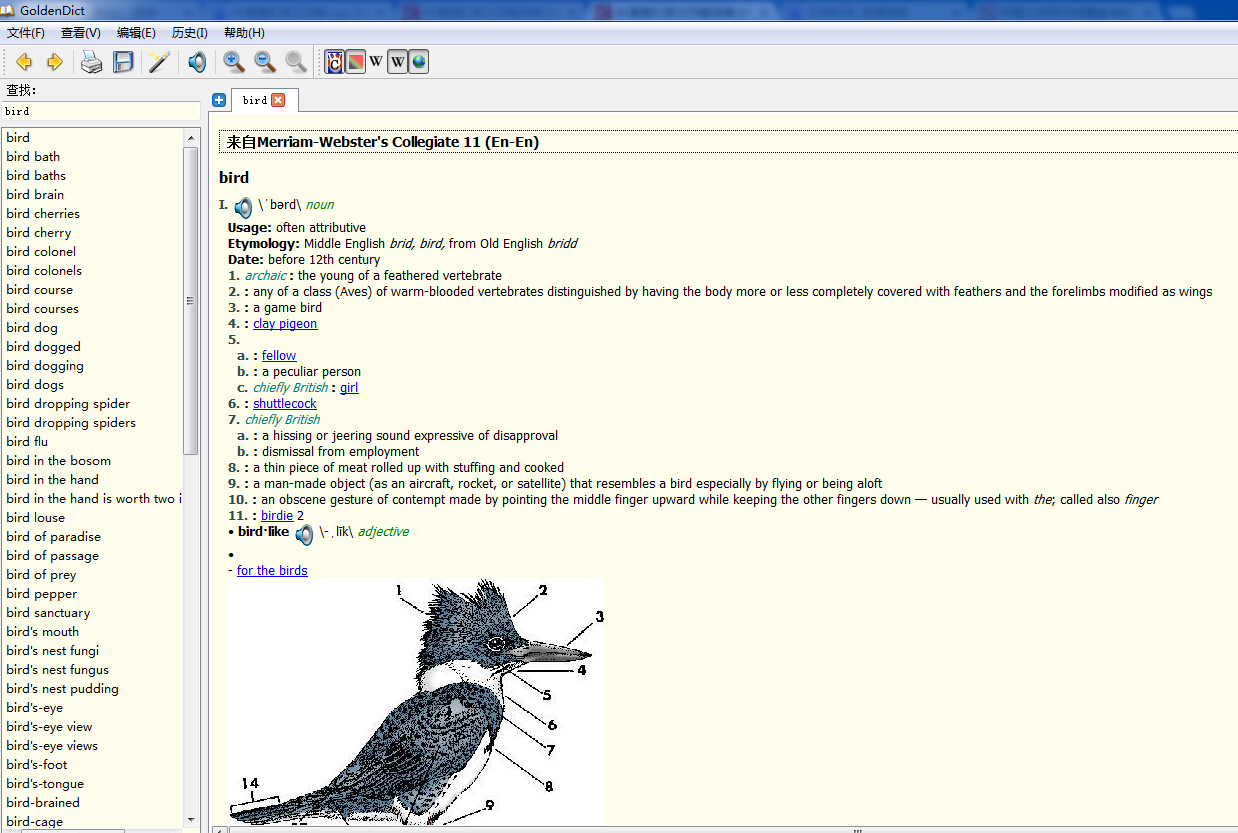
\includegraphics[scale=0.35]{GoldenDictWebster.jpg}
		\caption{GoldenDict韦伯英英词典}
		\label{GoldenDictWebster}
	\end{figure}
	
	Longman Pronunciation Dictionary 3rd edition(En-En)-朗文发声辞典第三版,词典中有英音、美音,并对于“多音”的词,配有preference poll图表,即不同的发音在不同地区、不同年龄层里所占的比例。  
	
	Longman DOCE5-Longman Dictinary of Contemporary English 5th edition(En-En)-朗文当代第五版英英词典,含发音和图片,大部分例句也带有朗读。  
	
	Longman DOCE5 Extras(En-En)-不包含单词发音和图片,但是包含了该词汇的各种搭配,和牛津搭配词典类似
	
	牛津高阶英汉双解 第四版(En-zh\_CN)-英汉双解,我想这个对于国人是必不可少,bgl的格式,排版很美观,无发音,如图\ref{GoldenDictOxford}所示。   
	
	\begin{figure}[htbp]
		\centering
		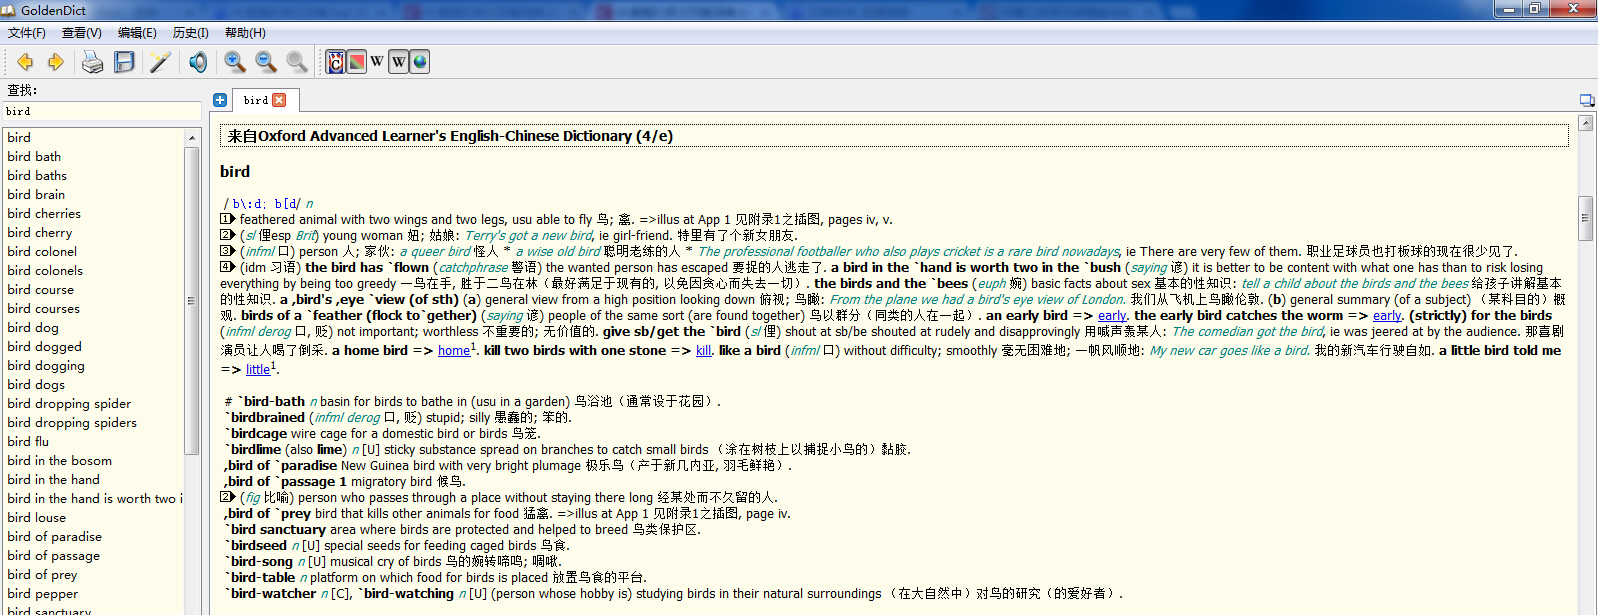
\includegraphics[scale=0.35]{GoldenDictOxford.jpg}
		\caption{GoldenDict牛津高阶英汉词典}
		\label{GoldenDictOxford}
	\end{figure}
	
	\clearpage
		
	\part{程序开发}	
	
	\clearpage
	
	作为IT行业程序开发的技能大致有:
	\begin{itemize}
		\item{RDBMS Management}~~RDBMS(关 系数据库管理系统)是一个行业数据。这是一种很传统的数据库,使用了SQL语言,被甲骨文、微软SQL Server和IBMDB2等数据库广泛使用。虽然新一代NoSQL数据库应用增长飞快,但多数公司仍在使用这一种技术来处理最重要的企业应用。
		\item{JDBC}~~JDBC 是甲骨文基于Java开发的一种技术,它可以帮助数据库连接一个用Java语言编写的应用。Java是常见的应用编程语言。
		\item{Sqoop}~~Sqoop 的流行得益于大数据浪潮的兴起。这是一种免费的开源工具,可以帮助你将数据从流行的大数据存储系统Hadoop转移到经典的关系数据库中(例如甲骨文、 IBM和微软的数据库)。这是一种命令行界面工具,因此你必须知道各种命令,并直接键入系统,而不能使用鼠标点击来操作。
		\item{UML}~~当今的软件都太复杂了,但UML(统一建模语言)解决了这个问题。这是一种视觉化的语言,将复杂的软件设计转变成易于理解的范式。
		\item{Documentum}~~EMCDocumentum是一套“企业内容管理”系统,可以方便企业存储和搜索各类文件。虽然Hadoop等大数据应用提供了新时代的数据处理方案,但Documentum在很多仍需使用大量纸质和电子文档的行业仍然很受欢迎,包括法律、医疗和保险等行业。
		\item{大数据技术}~~大 数据是一种新型海量数据分析软件,它们可以处理各种格式的信息,包括推文、博文、电子邮件、文档、音频、视频等。现在有越来越多的技术开始融入“大数据世 界”,包括各种分析软件、记忆型数据库、NoSQL数据库、Hadoop等。创业公司、科技巨头各类企业都在争相融入这一浪潮。
		\item{SOA}~~SOA其实是一个很老的软件概念,但得益于云计算的发展而再次流行。它的意思是“服务导向架构”,这种技术的实施者会编写一些小服务,以便在不同的应用之间共享。例如,云计算应用不必自主处理密码,而是可以通过共享的“密码服务”来实现这项功能。
		\item{Hadoop}~~Hadoop是大数据时代的核心技术。这是一种开源软件,可以汇总和存储海量信息,并以低成本的通用硬件对其进行分析。例如,银行可以使用Hadoop来探测虚假信息,而购物网站也可以使用它来分析用户购买习惯。
	\end{itemize}
	
	
	\newpage
	
	\section{DBeaver}
	
	\subsection{简介}
	
	DBeaver is free and open source (GPL) universal database tool for developers and database administrators.
	
	Usability is the main goal of this project, program UI is carefully designed and implemented.
	It is freeware.
	It is multiplatform.
	It is based on opensource framework and allows writing of various extensions (plugins).
	It supports any database having a JDBC driver.
	It may handle any external datasource which may or may not have a JDBC driver.
	There is a set of plugins for certain databases (MySQL and Oracle in version 1.x) and different database management utilities (e.g. ERD).
	
	\subsection{配置}
	
	\begin{figure}[htbp]
		\centering
		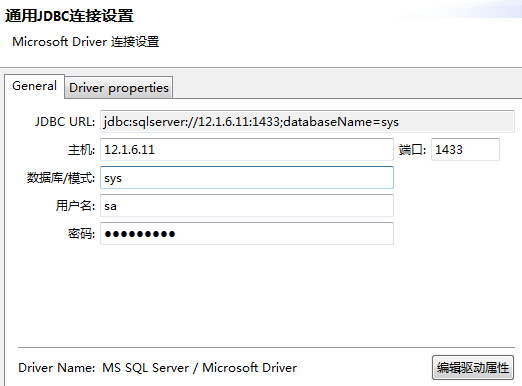
\includegraphics[scale=0.8]{JDBCConnectionConfig.jpg}
		\caption{DBeaver配置}
		\label{JDBCConnectionConfig}
	\end{figure}
	
	\section{Git}
	Git is a fast, scalable, distributed revision control system with an unusually rich command set that provides both high-level operations and full access to internals.
	
	\subsection{Git使用}
	
	查看当前版本库的状态,使用git status命令,如图\ref{GitRepositoryStatus}所示。此时提示工作区的内容有被修改过。使用git diff命令查看文件修改前后的对比,如图\ref{GitDiffFileOperation}所示。
	
	\begin{figure}[htbp]
		\centering
		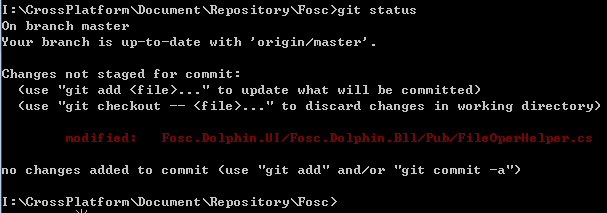
\includegraphics[scale=0.8]{GitRepositoryStatus.jpg}
		\caption{查看Git库状态}
		\label{GitRepositoryStatus}
	\end{figure}
	
	
		\begin{figure}[htbp]
			\centering
			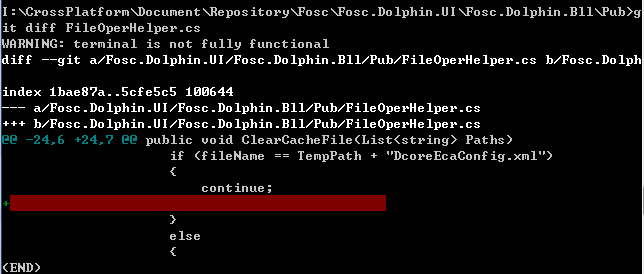
\includegraphics[scale=0.8]{GitDiffFileOperation.jpg}
			\caption{文件修改对比}
			\label{GitDiffFileOperation}
		\end{figure}
	\section{make}	
	
	需要将改动后的文件添加到版本库中,使用命令:git add OpenSourceSoftware.aux。提交所有改动,使用命令git commit -m "commit"。
	
	\subsection{Linux下编译源码}	
	
	切换到源码目录下,这里以Audacity\footnote{http://en.wikipedia.org/wiki/Audacity\_(audio\_editor)}的原始码为例,执行configure命令,如图\ref{ConfigureCommand}所示。	
	
	\begin{figure}[htbp]
		\centering
		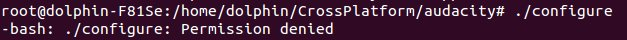
\includegraphics[scale=0.8]{ConfigureCommand.jpeg}
		\caption{Configure}
		\label{ConfigureCommand}
	\end{figure}
	
	执行命令时会提示错误,-bash: ./configure: Permission denied。错误的原因是此时configure文件没有可执行权限。将文件添加可执行权限,如图\ref{ChangeModCommand}所示。	
	
	\begin{figure}[htbp]
		\centering
		
\includegraphics[scale=0.8]{ChangeModCommand.jpeg}
		\caption{添加文件权限}
		\label{ChangeModCommand}
	\end{figure}
		
	\clearpage
	\part{软件使用}
	\clearpage
	\section{Gmail}
	
	
	
	
	\clearpage
	\part{附录}
	\clearpage
	\section{词汇}
	\begin{tabular}{ll}			
		\multirow{1}{*}{\textbf{中文}}			
		& \multicolumn{1}{l}{\textbf{英文}}\\			
		硫酸纸 & Tracing Paper\\
		专业 & Discipline\footnotemark[1]\\
	\end{tabular}
	\footnotetext[1]{参照:A/E/C CAD Standard Release 5.0}		
	\clearpage	
\end{document}